\documentclass[main.tex]{subfiles}
\begin{document}



\chapter{Background}

% TODO
% - terminologie compilation toolchain
% - infer block ram during compilation

\section{Field-programmable gate arrays}
Field-programmable gate arrays (FPGAs) are a class of integrated circuits (IC) which' behaviour is reconfigurable, as opposed to application specific integrated circuits (ASIC). In their most common form, FPGAs consist of blocks of configurable logic which are interconnected through a configurable network. Many manufacturers combine CLBs with additional static functionality such as memories, I/O controllers and even embedded microprocessors. Which static features are included differs per FPGA model and manufacturer. Figure \ref{fig:fpgastructure} gives a structural overview of a FPGA as manufactured by Xilinx. It shows a number of CLBs, interconnected with I/O blocks (IOB) that connect IC package pins and block rams (BRAM) which serve as static blocks of memory. The digital clock manager (DCM) is responsible for the distribution of clock signals to every of the FPGA's blocks. 

A CLB's contained logic is described through an internal lookup table in which 

\begin{figure}
\centering
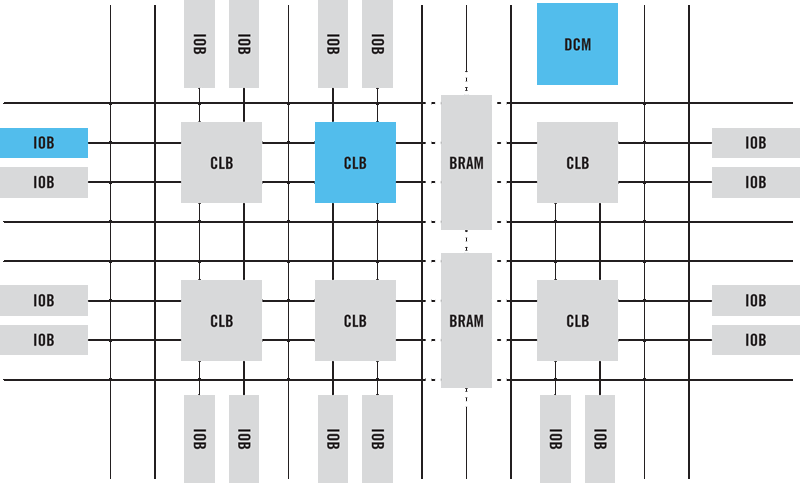
\includegraphics[width=.7\textwidth]{img/fpga-block-structure}
\caption{Structural FPGA overview}
\label{fig:fpgastructure}
\end{figure}

\begin{figure}
\centering
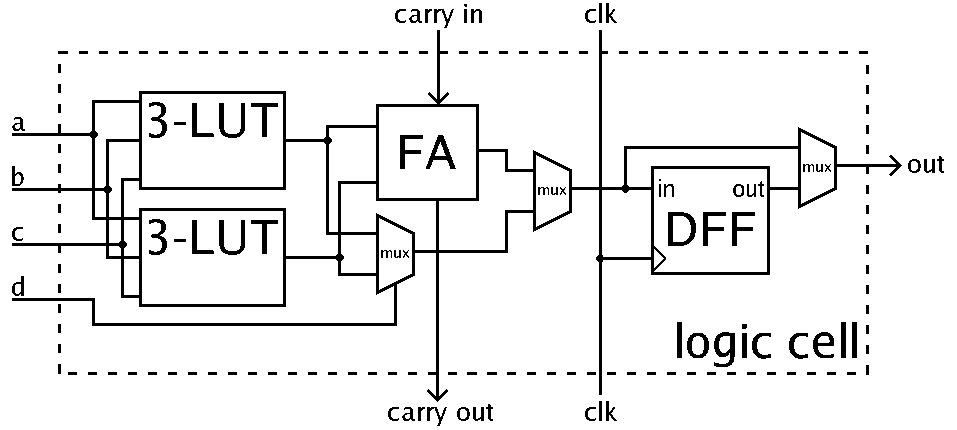
\includegraphics[width=.7\textwidth]{img/fpga-clb}
\caption{FPGA CLB example overview}
\label{fig:my_label}
\end{figure}



\subsection{I/O capabilities}
A FPGA development board generally includes a number of I/O devices. Simple devices for input include buttons and switches, while simple output devices are generally LEDs or LED displays. Furthermore, a development board often includes a set of pin headers, which can be configured individually to be input or output ports. 

More complex I/O devices are included as well. Such as VGA output controllers, microphone, Ethernet, USB, .... These devices operate within strict timing constraints in order to work properly. This prevents the experiment setup from properly using the device, since it runs on a irregular, low frequency. 

Buffering (right term?) of some types of input, such as push buttons. When a user presses a push button while the experiment is halted, the signal should be artificially set to be high during the next cycle.

I/O devices can only be seen as combinational circuits. I/O devices that are based on sequential logic, such as a LED display controller, an abstraction needs to be created such that the device behaves like a combinational circuit. 

\subsection{Programming}
Generally speaking, FPGA development board come equipped with dedicated hardware for the purpose of programming. 

% Current FPGAs generally make use of the IEEE 1532 standard for in-system programming, which extends the IEEE 1149.1 'JTAG' boundary scan protocol. In order to program these FPGAs, one makes use of dedicated JTAG programming hardware and software. Such hardware and software is commonly available.  

% FPGA development board manufacturers generally integrate JTAG programming hardware in their designs, allowing progamming over a serial connection to their PC, such as USB. Manufacturers combine their development boards with software development kits that facilitate the operating system drivers and software required for the programming process. Other means of programming are seen as well, such as support for USB storage devices or memory cards on which a file is placed that is automatically read by the development board and programmed onto the FPGA. FPGA development boards generally feature a JTAG interface as well, allowing for a custom method of programming using external tools. 

\subsection{PC Communication}
In order to allow for communcation with a PC, FPGA development board manufacturers generally include one or more communication interfaces in their board designs. Many FPGA development boards currently available come with a USB interface over which a virtual serial interface is exposed, commonly known as a virtual COM port. The serial signal is often controlled by a UART implementation that is programmed onto the FPGA. Other examples of communcation interfaces are RS232 and Eternet ports, where dedicated hardware components on the FPGA development board are responsible for translating signal levels controlled in the FPGA to interface standard levels. 


\subsection{Clock Distribution}

\section{FPGA Development Toolchain}

\subsection{Synthesis}
Synthesis is the process of translating a HDL design to a desired primitive unit. Logic gates, CLB's.

\subsection{Place \& Route}

\subsection{Bitstream Generation}

\section{Software Development Kits}

\section{Hardware Description Languages}


% FPGA
% Eductional
% Computer architecture
% PC
% Instruction level view
% MIPS 

% Introduction
% Problem description
% Related work
% Educational softcores
% 
% FPGA fundamentals
% - toolchain
% 


\end{document}